
\section{Layout of the Endcap Petal}

Figure~\ref{endcap_model} depicts the endcap petal model used for calculating thermal impedances.

\begin{figure}[ht!]
\begin{center}
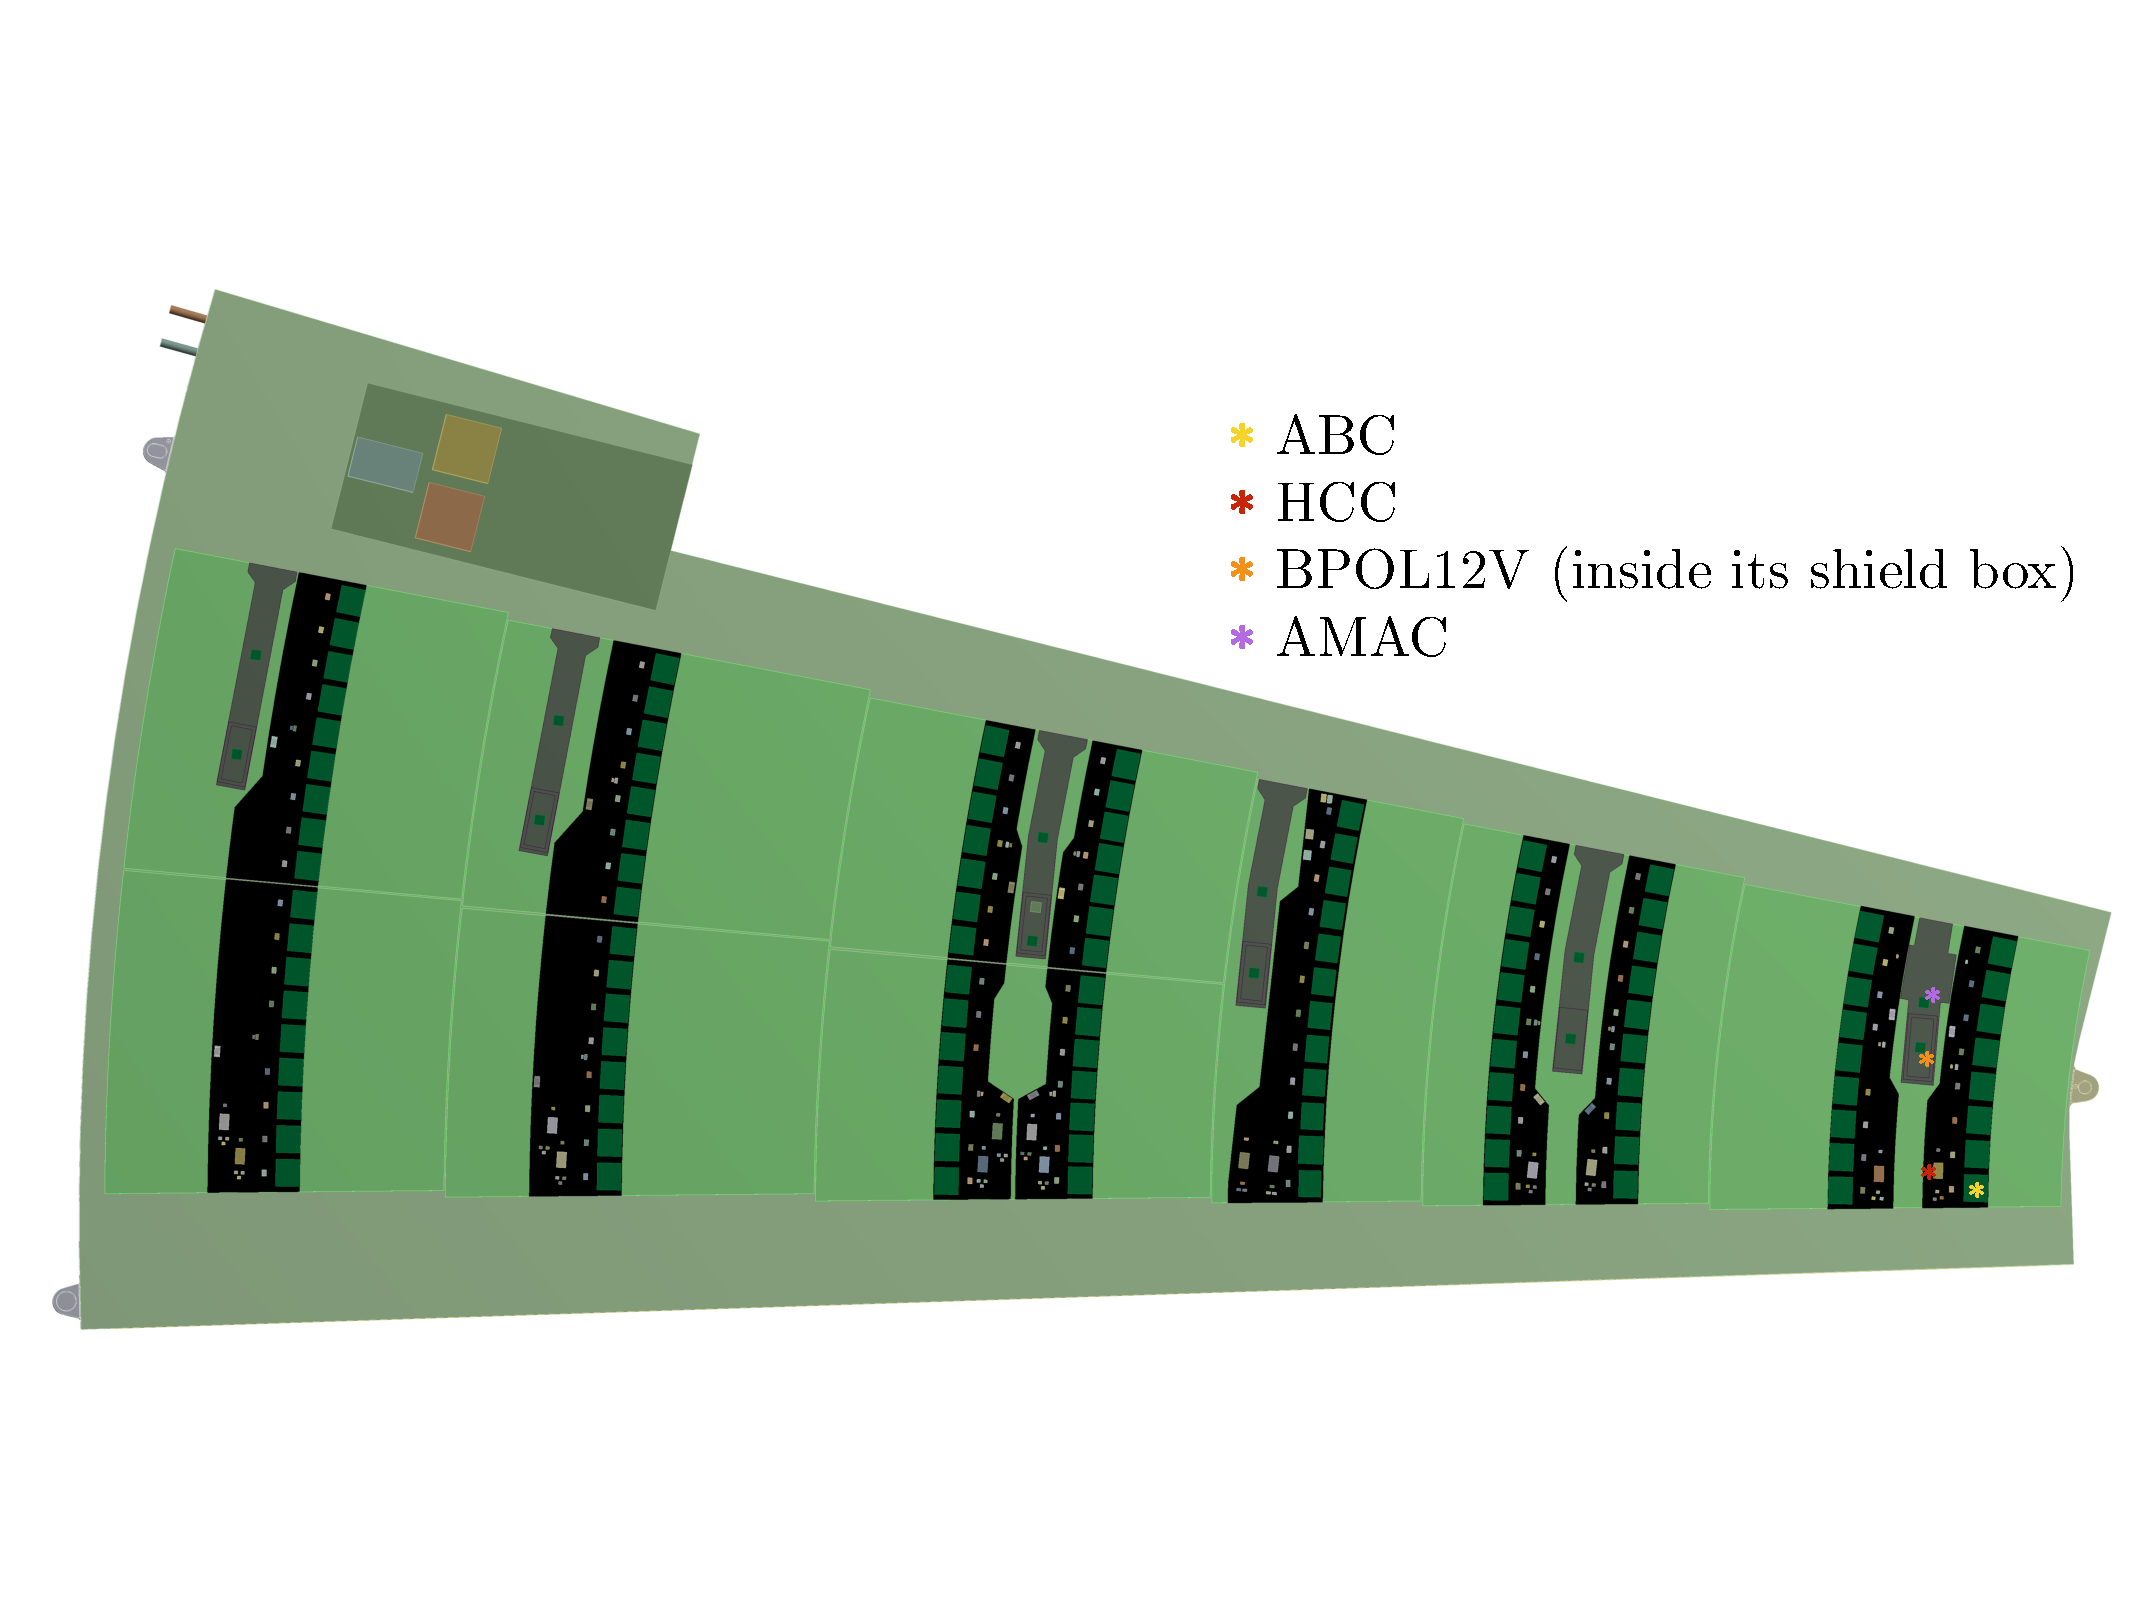
\includegraphics[width=0.99\linewidth]{figures/m30C_0Wm2C_Setup_BPOL12V.pdf}
\end{center}
\caption{The endcap petal model used for extracting thermal impedances. The front-end components are
labeled in R0 (the rightmost module).}
\label{endcap_model}
\end{figure}

The number of BPOL12Vs, AMACs, ABCs, HCC, and the sensor area of each module are listed in
Table~\ref{tab:layout_parameters}.
%
\let\arraystretcha\arraystretch
\renewcommand\arraystretch{1.1} % 1.6
\begin{table}[h]
\begin{center}
\adjustbox{max width=\textwidth}{ %% just before tabular
\begin{tabular}{|l|r|r|r|r|r|r|} \hline
Module & nBPOL12V & nAMAC & nABC & nHCC & Sensor area (cm$^2$) \\ \hline
R0     &      1 &     1 &   17 &    2 &                 92.0 \\
R1     &      1 &     1 &   21 &    2 &                 91.0 \\
R2     &      1 &     1 &   12 &    2 &                 76.0 \\
R3     &      2 &     2 &   28 &    4 &                164.0 \\
R4     &      1 &     1 &   16 &    2 &                178.0 \\
R5     &      1 &     1 &   18 &    2 &                186.0 \\
\hline \end{tabular}
} %% resizebox after tabular
\end{center}
\caption{Number of components on each module. The sensor area refers to the total sensor area, e.g.
for R3, R4, and R5 it refers to the sum of the two sensors on the module.}
\label{tab:layout_parameters}
\end{table}
\let\arraystretch\arraystretcha

Note that the sensor area quoted above refers to the total sensor area. For R3, R4, and R5, which
consist of two sensors, this means the total area of the two sensors. More details of how those sensors
are treated in the model is described in Section~\ref{highvoltage}.
